\chapter{Supplemental Information}\label{app:supplemental-information}

%\begin{itemize}
%    \setlength\itemsep{0.4cm}
%    \item \textbf{wifi:} options for wifi
%        \begin{itemize}
%            \item \textbf{activate:} open up a hotspot - runs wifiActivate.sh
%                \subitem \textbf{choose the wifi standard}
%            \item \textbf{deactivate:} turn off the active network - runs wifiReset.sh
%            \item \textbf{status:} display the current networks settings - runs wifiStatus.sh
%            \item \textbf{change password:} set new password for a network - runs wifiNewPassword.sh
%                \subitem \textbf{choose the wifi standard}
%            \item \textbf{monitoring:} settings for wifi monitor - runs wifiMonitor.sh
%                \subitem \textbf{on} 
%                \subitem \textbf{off}
%                \subitem \textbf{show log}
%                \subitem \textbf{delete log}
%        \end{itemize}
%    \item \textbf{webapp:} options for webapps
%        \begin{itemize}
%            \item \textbf{Juice Shop:} settings for the Juice Shop - runs juiceShop.sh
%                \subitem \textbf{on}
%                \subitem \textbf{off}
%            \item \textbf{MQTT:} settings for MQTT communication - runs mqtt.sh and the mqtt program
%                \subitem \textbf{on}
%                \subitem \textbf{off}
%        \end{itemize}
%    \item \textbf{development:} runs development options from XXX.sh
%    \item \textbf{power off:} power off the system - runs shutdown.sh
%\end{itemize}

\section{User Manual}
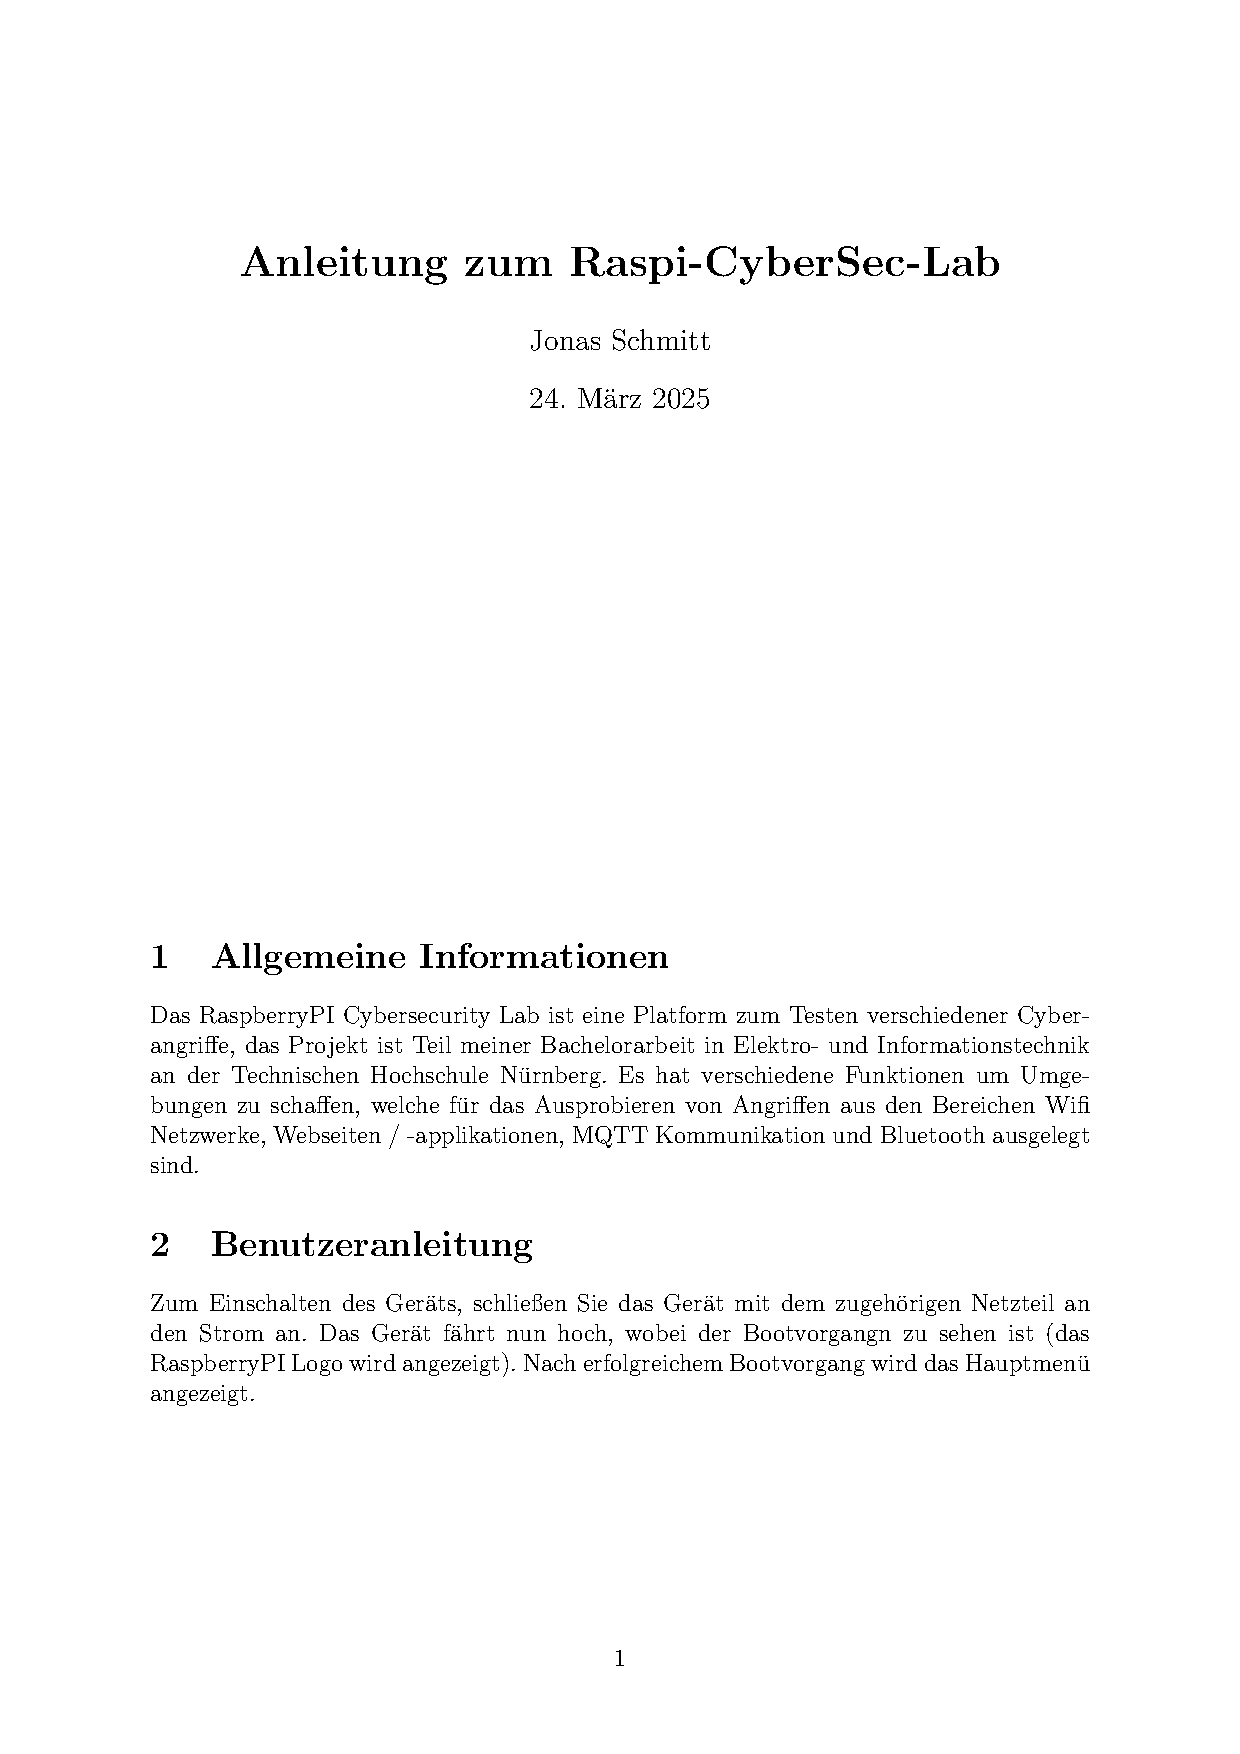
\includepdf[pages={1-}]{userguide/userguide.pdf}

\section{Documentation}
\begin{table}[h]
    \caption{menu and option overview}
    \label{tab:menues_options}
    \centering
    \ra{1.3}
    \small
        \begin{tabular}{@{}lrclclrclcl@{}}\toprule
            \multicolumn{11}{c}{Main Menu} \\
            \midrule
            \multicolumn{2}{c}{wifi} && \multicolumn{1}{c}{bluetooth} && \multicolumn{2}{c}{webapp} && development && power off \\
            \cmidrule{1-2} \cmidrule{4-4} \cmidrule{6-7} \cmidrule{9-9} 
            activate & WEP && \textit{under} && Juice Shop & on && option 1 && \\
            & WPA && \textit{development} &&& off && option 2\\
            & WPA2 &&&& MQTT & on && option 3\\
            & WPA3 &&&&& off && option 4\\
            deactivate &&&&&&&& option 5\\
            status\\
            new password & WEP\\
            & WPA\\
            & WPA2\\
            & WPA3\\
            monitor & on\\
            & off\\
            & show log\\
            & delete log\\
            \bottomrule
        \end{tabular}
\end{table}


\begin{figure}[h]
    
\includegraphics[width=0.25\linewidth]{figures/Abbildungen/hackerypi/menu_wifi.png}
    
\includegraphics[width=0.3\linewidth]{figures/Abbildungen/hackerypi/menu_webapp.png}
    
\includegraphics[width=0.35\linewidth]{figures/Abbildungen/hackerypi/menu_dev.png}
    \centering
    \caption{Device Menues}
    \label{fig:menues}
\end{figure}